\documentclass[]{article}
\usepackage{standalone}\standalonetrue
\ifstandalone
  \usepackage{../../haziq_article}
  \usepackage{../../knitr}
  \addbibresource{../../library.bib}  
\fi
\begin{document}

\ifstandalone{

%%%%%%%%%%%%%%%%%%%%%%%%%%%%%%%%%%%%%%%%%%%%%%%%%%%%%%%%%%%%%%%%%%%%%%%%%%%%%%%%
%%% TO-DO LIST %%%%%%%%%%%%%%%%%%%%%%%%%%%%%%%%%%%%%%%%%%%%%%%%%%%%%%%%%%%%%%%%%
%%%%%%%%%%%%%%%%%%%%%%%%%%%%%%%%%%%%%%%%%%%%%%%%%%%%%%%%%%%%%%%%%%%%%%%%%%%%%%%%
\pagenumbering{roman}
\listoftodos[To-do list]
\newpage

%%%%%%%%%%%%%%%%%%%%%%%%%%%%%%%%%%%%%%%%%%%%%%%%%%%%%%%%%%%%%%%%%%%%%%%%%%%%%%%%
%%% TITLE %%%%%%%%%%%%%%%%%%%%%%%%%%%%%%%%%%%%%%%%%%%%%%%%%%%%%%%%%%%%%%%%%%%%%%
%%%%%%%%%%%%%%%%%%%%%%%%%%%%%%%%%%%%%%%%%%%%%%%%%%%%%%%%%%%%%%%%%%%%%%%%%%%%%%%%
\title{Multinomial probit I-prior models}
\author{
  Haziq Jamil\\
  \normalsize{\it{Department of Statistics}}\\
  \normalsize{\it{London School of Economics and Political Science}}
}
\date{\normalsize\today}
\maketitle
%{\let\newpage\relax\maketitle}  % if need some text before the title use this
%\pagenumbering{roman}

%%%%%%%%%%%%%%%%%%%%%%%%%%%%%%%%%%%%%%%%%%%%%%%%%%%%%%%%%%%%%%%%%%%%%%%%%%%%%%%%
%%% ABSTRACT %%%%%%%%%%%%%%%%%%%%%%%%%%%%%%%%%%%%%%%%%%%%%%%%%%%%%%%%%%%%%%%%%%%
%%%%%%%%%%%%%%%%%%%%%%%%%%%%%%%%%%%%%%%%%%%%%%%%%%%%%%%%%%%%%%%%%%%%%%%%%%%%%%%%
\begin{abstract}
Extension of I-prior models to multi-class classification with estimation using variational inference.

\vspace{1em}
{\noindent\textbf{Keywords:} 
	some, keywords, go, here
}
\end{abstract}
}
\fi
\pagenumbering{arabic}

\section{Introduction}

Consider multinomial response variables $y_1, \dots, y_n$, where each response $y_i$ takes on one of the values $\{1,\dots,m\}$ from a set of $m$ possible values. We model each response as following a categorical distribution (a special case of the multinomial distribution)
\[
  y_i \sim \Mult(p_{i1}, \dots, p_{im}),
\]
with probability mass function (pmf)
\[
  p(y_i) = p_{i1}^{\ind[y_i = 1]} \cdots p_{im}^{\ind[y_i = m]},
\]
such that $p_{ij} \geq 0 $ for each $j$ and $\sum_{j=1}^m p_{ij} = 1$. It might also be convenient to think of the responses $y_i$ as comprising of a binary vector of length $m$, with a single `1' at the position corresponding to the value that $y_i$ takes. That is,
\[
  y_i = (y_{i1}, \dots, y_{im})
\]
with
\[
  y_{ik} =
  \begin{cases}
    1 &\text{ if } y_i = k \\
    0 &\text{ if } y_i \neq k
  \end{cases}
\]
and $\sum_{j=1}^m y_{ij} = 1$. In this formulation, each $y_{ij}$ is distributed as Bernoulli with probability $p_{ij}$.

Suppose for each observation $y_i$ there is an associated $p$-dimensional vector of covariates $x_i = (x_{i1}, \dots, x_{ip})$ belonging to some set $\cX$. We would like to model the multinomial outcomes $y_i$ based on these vectors of covariates. Assume that for each $y_i = (y_{i1}, \dots, y_{im})$, there exists a corresponding continuous, underlying, latent variable $y_i^* = (y_{i1}^*, \dots, y_{im}^*)$ such that
\[
  y_i =
  \begin{cases}
    1 &\text{ if } y_{i1}^* \geq y_{i2}^*, y_{i3}^*, \dots, y_{im}^* \\
    2 &\text{ if } y_{i2}^* \geq y_{i1}^*, y_{i3}^*, \dots, y_{im}^* \\
    \vdots \\
    m &\text{ if } y_{im}^* \geq y_{i2}^*, y_{i3}^*, \dots, y_{i\,m-1}^*. \\
  \end{cases}
\]
In other words, 
\[
  y_{ij} = \ind[y_{ij}^* = \max_k y_{ik}^*].
\]

We consider modelling the $n$ latent variables in each class $j=1,\dots,m$ according to the regression problem
\begin{equation}\label{eq:multinomial-latent}
  \begin{gathered}
    y_{ij}^* = f_j(x_i) + \epsilon_{ij} \\
    \epsilon_{ij} \iid \N(0, \sigma_j^2) \\
    i = 1,\dots,n
  \end{gathered}
\end{equation}
with $f_j:\cX \to \bbR$ being a regression function belonging to some reproducing kernel Hilbert space of functions $\cF_j$ having the reproducing kernel $h_{\lambda_j}: \cX \times \cX \to \bbR$. Here, $\lambda_j$ is the scale parameter for the reproducing kernel, so that $h_{\lambda_j}(\cdot) = \lambda_j h(\cdot)$. One advantage of the multinomial probit model is the ability to also model the correlations across choices, such that for each $j,k \in \{1,\dots,m\}$ and $j \neq k$,
\[
  \Corr[\epsilon_{ij}, \epsilon_{ik}] = \frac{\sigma_{jk}}{\sigma_j \, \sigma_k}.
\]
This setting is suitable for modelling multinomial data where the independence axiom is not desired. Such cases arise frequently in economics and social science. The famous Red-Bus-Blue-Bus example is often used to illustrate independence of irrelevant alternatives (IIA). Suppose commuters face the decision between taking cars and red busses. The addition of blue busses to commuters' choice should not affect the choice between cars or busses (assuming commuters are indifferent about the colour of the bus). Yet, if IIA is imposed, then the three choices are distinct, and the fact that red and blue busses are substitutable is ignored.

The IIA assumption is realised by fixing $\sigma_{jk} = 0$, $j \neq k$, which is clearly a simplification of the model (and as we will see later, benefits us in the algebra when deriving some distributional results). As this may not be suitable for certain modelling purposes, we might want to consider how this assumption can be relaxed, but we leave this for future work. 

Back to model \eqref{eq:multinomial-latent}: We wish to model the function $f_j$ as having an I-prior. Denoting $f_{ij} = f_j(x_i)$ as the evaluation of the function $f_j(\cdot)$ at $x_i$, and also $\bff_j = (f_{1j}, \dots, f_{nj})^\top$ as the vector containing all $n$ evaluations pertaining to the $j$th alternative, an I-prior on $f_j$ is 
\[
  \bff_j \sim \N(\bff_j^0, \cI_j)
\]
where $\cI_j$ is the $n \times n$ Fisher covariance kernel for the regression function $f_j$ in model \eqref{eq:multinomial-latent}, which has $(r,s)$ entries given by
\[
  \cI_j\big( f_j(x_r), f_j(x_s) \big) = \sigma_j^{-2} \sum_{k=1}^n \sum_{l=1}^n  h_{\lambda_j}(x_r, x_k) h_{\lambda_j}(x_l, x_s)
\]
and $\bff_j^0$ is a vector of prior means. By concatenating the vectors $\bff_1, \dots, \bff_m$ into the vector $\bff$ of length $nm$, it is easy to see that 
\[
  \bff \sim \N(\bff^0, \bOmega)
\]
where $\bff^0 = (\bff_1^0, \dots, \bff_m^0)^\top$ and $\bOmega = \diag(\cI_1, \dots, \cI_m)$. This stems from the fact that the error components are independent across choices (IIA), and as such, $\Cov[\bff_j, \bff_k] = \bzero$, $j \neq k$. In the more general case where $\sigma_{jk} \neq 0$, then extra care must be taken to ensure the covariances are represented in the I-prior covariance matrix.

We make two further simplifications to the model. Firstly, the choice model as stated is not identified in scale, i.e. multiplication of the latent variables by a positive constant does not make any difference to the outcome. This is a well known identification issue\footnotemark with the multinomial probit model, and this is typically overcome by setting some restrictions. In our case, we set all $\sigma_j^2 = 1$.\hltodo[But isn't identifiability resolved by setting all covariances to zero?]{}

\footnotetext{In the unrestricted case for a model with $m$ alternatives, there would be $m(m+1)/2$ variance components to estimate. However, in general, only $m(m-1)/2$ can be freely estimated.}

Secondly, we assume that the intercept functions (prior means) are constants, so that $\bff^0_j = \alpha_j\bone_n$ for $j=1,\dots,m$, and the $\alpha_j$s are just additional hyperparameters to be estimated. With all of these in mind, the I-prior model simplifies to
\begin{gather*}
  y_{ij}^* = \alpha_j + \sum_{k=1}^n h_{\lambda_j}(x_i, x_{k})w_{kj} + \epsilon_{ij} \\
  \epsilon_{ij} \iid \N(0,1) \\
  w_{kj} \iid \N(0,1) 
\end{gather*}
for each $j \in \{1,\dots,m\}$. Define $f_{ij} = \alpha_j + \sum_{k=1}^n h_{\lambda_j}(x_i, x_{k})w_k$, so that each $y_{ij}^*|f_{ij} \sim \N(f_{ij}, 1)$. The probit link is seen as follows:
\begin{align*}
  p_{ij} 
%  &= \Prob[y_i = j] \\
%  &= \Prob[y_{ij} = 1] \\
  &= \Prob\left[y_{ij}^* = \max_k y_{ik}^* \right] \\
  &= \Prob\left[y_{ij}^* > y_{ik}^* : \forall k \neq j \right] \\
  &= \Prob\left[ 
  f_{ij} + \epsilon_{ij} > f_{ik} + \epsilon_{ik} : \forall k \neq j
   \right] \\
  &= \Prob\left[\epsilon_{ik} - \epsilon_{ij} \leq f_{ij} - f_{ik} : \forall k \neq j \right] \\
  &= \idotsint \ind\left[\epsilon_{ik} \leq \epsilon_{ij} + f_{ij} - f_{ik} : \forall k \neq j \right]
  \prod_{k=1}^m \big[ \phi(\epsilon_{ik}) \d\epsilon_{ik} \big] \\
  &= \int \mathop{\prod_{k=1}^m}_{k\neq j} \Phi(\epsilon_{ij} + f_{ij} - f_{ik})
    \phi(\epsilon_{ij}) \d\epsilon_{ij} \numberthis \label{eqn:probit-link} \\
  &= \E_Z \Bigg[ \mathop{\prod_{k=1}^m}_{k\neq j} \Phi(Z + f_{ij} - f_{ik}) \Bigg]
%  &= \mathop{\prod_{k=1}^m}_{k\neq j} \Phi \left( e_k \right) 
\end{align*}
where $Z$ is a standard normal random variable, and $\phi(\cdot)$ and $\Phi(\cdot)$ are the pdf and cdf of a standard normal distribution respectively. \hltodo[Citation?]{It is well know that for $m>3$ this has no closed form expression, which makes the probit model unattractive from a likelihood maximisation standpoint.}

%\begin{lemma}\label{lem:EPhiZ} 
%  Let $Z \sim \N(0,1)$. Then 
%  \[
%    \E[\Phi(z)] = 1/2.
%  \]
%\end{lemma}
%
%\begin{proof}
%  Define the random variable $Y$ by $Y = \Phi(Z)$. Note that $Y \in [0,1]$, and is monotonically increasing within this interval. Then,
%  \begin{align*}
%    F(y) &= \Prob[Y \leq y] \\
%    &= \Prob[\Phi(Z) \leq y] \\
%    &= \Prob[Z \leq \Phi^{-1}(y)] \\
%    &= \Phi\big( \Phi^{-1}(y) \big) = y
%  \end{align*}
%  which implies that $Y$ is uniform in the interval $[0,1]$. Thus,
%  \[
%    \E[\Phi(Z)] = 1/2.
%  \]
%\end{proof}

%\begin{lemma}\label{lem:expectation-of-prod-phi}
%  Let $Z \sim \N(0,1)$. Then, for $\sigma > 0$,
%  \[
%    \E_Z \left[ \prod_{i=1}^n \Phi(\mu_i + \sigma_i Z) \right] = \prod_{i=1}^n \Phi \left(e_i \right).
%  \]
%  where $e_i$ are the elements of $\be = \bL^{-1} [\mu_1 \cdots \mu_n]^\top$, and $\bL$ is the Cholesky decomposition of the $n\times n$ matrix $\bSigma = [\sigma_1 \cdots \sigma_n] \otimes [\sigma_1 \cdots \sigma_n] + \bI_n$.
%\end{lemma}
%
%\begin{proof}
%Let $Z, Z_1, \dots, Z_n$ denote standard normal random variables independent of each other. Then 
%  \begin{align*}
%    \E_Z \left[ \prod_{i=1}^n \Phi(\mu_i + \sigma_i Z) \right]
%    &= \int \prod_{i=1}^n \Phi(\mu_i + \sigma_i z) \phi(z) \d z \\
%    &= \idotsint \ind[z_i < \mu_i + \sigma_i z: \forall i] \, \phi(z_1) \cdots \phi (z_n) \phi(z) \d z_1 \cdots \d z_n \d z \\
%    &= \Prob \left[Z_i < \mu_i + \sigma_i Z: \forall i \right] \\
%    &= \Prob \left[Z_i - \sigma_i Z < \mu_i: \forall i \right] \\
%  \end{align*}
%  Now if we define new random variables $U_i = Z_i - \sigma_i Z$ then each $U_i$ will be normally distributed with mean 0 and variance $1 + \sigma_i^2$. The covariance between any two pair of random variables $U_i$ and $U_j$ will be $\sigma_i\sigma_j$. Thus, the joint distribution of $\bU = (U_1, \dots, U_n)^\top$ is multivariate normal with mean $\bzero_n$ and covariance given by the $n \times n$ matrix $\bSigma = \bsigma \otimes \bsigma + \bI_n$, where $\bsigma = (\sigma_1, \dots, \sigma_n)^\top$, and $\otimes$ denotes the outer product. For a symmetric, positive-definite matrix such as $\bSigma$, we can obtain the Cholesky decomposition
%  \[
%    \bSigma = \bL\bL^\top
%  \]
%  where $\bL$ is lower-triangular. Now, if $\bW$ is a standardised $n$-variate normal distribution, then clearly $\bL\bW$ will have the same distribution as $\bU$. Thus, denoting $\bmu = (\mu_1, \dots, \mu_n)$,
%  \begin{align*}
%    \Prob \left[Z_i - \sigma_i Z < \mu_i: \forall i \right] 
%    &= \Prob[\bU < \bmu] \\
%    &= \Prob[\bL\bW < \bmu] \\
%    &= \Prob[\bW < \bL^{-1}\bmu] \\
%    &= \prod_{i=1}^n \Phi(e_i)
%  \end{align*}  
%  where $e_i$ are the elements of $\be = \bL^{-1}\bmu$.
%\end{proof}

The above describes $m$ regression functions being estimated for each class, and each of the $m$ regression functions estimated using an I-prior. It is possible for all $m$ regression functions\footnotemark to share a common I-prior $\bff_1, \dots, \bff_m \iid \N(\alpha\bone_n, \cI)$, so that only one set of intercept and RKHS scale parameters need to be estimated (instead of $m$ sets, one for each class). There is also flexibility in using the same covariance kernel for instance, but different intercepts for the $m$ I-priors, or vice-versa. The probit I-prior model can be represented by the following DAG.

\footnotetext{It is also possible to reparameterise the model (anchoring on one latent variable as the reference class and working with the latent differences) so that only $m-1$ I-priors are required.}

\begin{figure}[H]
  \centering
  \begin{tikzpicture}[scale=1.1, transform shape]
    \tikzstyle{main}=[circle, minimum size=10mm, thick, draw=black!80, node distance=16mm]
    \tikzstyle{connect}=[-latex, thick]
    \tikzstyle{box}=[rectangle, draw=black!100]
      \node[main, fill=black!10] (H) [] {$x_i$};
      \node[main, double, double distance=0.6mm] (f) [right=of H, xshift=1.2cm] {$f_{ij}$};
      \node[main, double, double distance=0.6mm] (ystar) [right=of f, xshift=1cm] {$p_{ij}$};
      \node[main] (lambda) [above=of f, xshift=-1.5cm, yshift=-0.3cm] {$\lambda_j$};        
      \node[main] (alpha) [above=of f, xshift=1.5cm, yshift=-0.3cm] {$\alpha_j$};  
      \node[main, fill = black!10] (y) [right=of ystar, xshift=0.2cm] {$y_{i}$};
      \node[main] (w) [below=of f] {$w_{ij}$};  
      \path (alpha) edge [connect] (f)
            (lambda) edge [connect] (f)
            (H) edge [connect] node [above] {$h$} (f)    		
    		(f) edge [connect] node [above] {probit} (ystar)
    		(ystar) edge [connect] (y)
    		(w) edge [connect] (f);
      \node[rectangle, draw=black!100, fit={(H) ($(y.north east) + (0,0.4cm)$) (w)}] {}; 
      \node[rectangle, fit= (w) (y), label=below right:{$i=1,\dots,n$}, xshift=0.15cm, yshift=0.5cm] {};  % the label
      \node[rectangle, draw=black!100, fit={(lambda) ($(ystar.north east) + (0.5cm,0.7cm)$) ($(w.south west) + (-0.5,-0.7cm)$)}] {}; 
      \node[rectangle, fit={(f) ($(ystar.north east) + (0.5cm,0.7cm)$) ($(w.south west) + (-0.5,-0.7cm)$)}, label=below right:{$j=1,\dots,m$}, xshift=-1.75cm, yshift=0.4cm] {}; 
    \end{tikzpicture}
    \caption{A DAG of the probit I-prior  model. Observed nodes are shaded, while double-lined nodes represented known or calculable quantities. The latent variables $y_{ij}^*$ have been marginalised and absorbed into the probit. The $w_{ij}$s are the standard normal random-effects associated with the I-prior. There are at most $m$ sets of intercept ($\alpha_j$) and scale ($\lambda_j$) parameters to estimate.}
\end{figure}

\section{Estimation}

The parameters to estimate in the probit I-prior model are $\btheta = (\alpha_1, \dots, \alpha_m, \lambda_1, \dots, \lambda_m)$. The likelihood function $L(\cdot)$ for $\btheta$ is obtained by integrating out the I-prior from the multinomial likelihood, as follows:
\begin{align*}
  L(\btheta) 
  &= \int \prod_{i=1}^n \prod_{j=1}^m p(y_i | f_{ij} ) \, p(f_{ij}|\alpha_j, \lambda_j) \d \bff \\
  &= \idotsint \prod_{i=1}^n \prod_{j=1}^m p_{ij}^{\ind[y_i = j]} \, p(\bff_j | \alpha_j, \lambda_j) \d \bff_1 \dots \d \bff_m .
\end{align*}
From \eqref{eqn:probit-link}, we know that $p_{ij}$ is related to the $f_{ij}$ via the integral involving the CDF and PDF of a standard normal. Thus, the intractable integral above presents a practical challenge which makes estimation via direct maximisation of the likelihood difficult to accomplish. Several approximations are considered, and discussed below.

\subsection{Laplace approximation}

\hltodo{Add section for Laplace's method}

\subsection{Markov Chain Monte Carlo}

\hltodo{Add section for MCMC}

\subsection{Variational inference}

\hltodo{Add section for variational inference}

\section{Estimation using variational inference}

The variational approximation to the probit I-prior model is made tractable by the inclusion of the latent variables $y_{ij}^*$ in the analysis as an intermediary step. The unknown quantities to estimate via variational inference are $y_{ij}^*$, $w_{ij}$, $\lambda_j$ and $\alpha_j$.

\begin{figure}[H]
  \centering
  \begin{tikzpicture}[scale=1.1, transform shape]
    \tikzstyle{main}=[circle, minimum size=10mm, thick, draw=black!80, node distance=16mm]
    \tikzstyle{connect}=[-latex, thick]
    \tikzstyle{box}=[rectangle, draw=black!100]
      \node[main, fill=black!10] (H) [] {$x_i$};
      \node[main, double, double distance=0.6mm] (f) [right=of H, xshift=1.2cm] {$f_{ij}$};
      \node[main] (ystar) [right=of f] {$y_{ij}^*$};
      \node[main] (lambda) [above=of f, xshift=-1.5cm, yshift=-0.3cm] {$\lambda_j$};        
      \node[main] (alpha) [above=of f, xshift=1.5cm, yshift=-0.3cm] {$\alpha_j$};  
      \node[main, fill = black!10] (y) [right=of ystar] {$y_{i}$};
      \node[main] (w) [below=of f] {$w_{ij}$};  
      \path (alpha) edge [connect] (f)
            (lambda) edge [connect] (f)
            (H) edge [connect] node [above] {$h$} (f)    		
    		(f) edge [connect] node [above] {} (ystar)
    		(ystar) edge [connect] (y)
    		(w) edge [connect] (f);
      \node[rectangle, draw=black!100, fit={(H) ($(y.north east) + (0,0.1cm)$) (w)}] {}; 
      \node[rectangle, fit= (w) (y), label=below right:{$i=1,\dots,n$}, xshift=-0.5cm, yshift=0.5cm] {};  % the label
      \node[rectangle, draw=black!100, fit={(lambda) ($(ystar.north east) + (0.5cm,0.7cm)$) ($(w.south west) + (-0.5,-0.7cm)$)}] {}; 
      \node[rectangle, fit={(f) ($(ystar.north east) + (0.5cm,0.7cm)$) ($(w.south west) + (-0.5,-0.7cm)$)}, label=below right:{$j=1,\dots,m$}, xshift=-2.05cm, yshift=0.2cm] {}; 
    \end{tikzpicture}
    \caption{A DAG of the variational probit I-prior  model.}
\end{figure}

\subsection{The joint likelihood}

\begin{align*}
  p(\by, \by^*, \bw, \lambda, \alpha)
  &= p(\by | \by^*, \bw, \alpha, \lambda) p(\by^*, \bff, \bw, \alpha, \lambda) \\
  &= p(\by|\by^*) p(\by^* | \bff) p(\bw) p(\lambda) p(\alpha)
\end{align*}

\subsection{Relevant distributions}

\begin{align*}
  p(\by|\by^*) &= \prod_{i=1}^n \prod_{j=1}^m p_{ij} 
  = \prod_{i=1}^n \prod_{j=1}^m \ind[y_{ij}^* = \max_k y_{ik}^*]^{\ind[y_i = j]} \\
  \\
  p(\by^*|\bff) &= \prod_{i=1}^n \prod_{j=1}^m \N(f_{ij},1) \\
  &= \exp \left[-\half[nm]\log 2\pi - \half \sum_{i=1}^n \sum_{j=1}^m (y_{ij}^* - f_{ij})^2 \right] \\
  &= \exp \left[-\half[nm]\log 2\pi - \half \norm{\by^* - \bff}^2 \right] \\
  \\
  f_{ij} &= \alpha_j + \sum_{k=1}^n  h_{\lambda_j}(x_i, x_k)w_{kj} \\
  \\
  p(\bw) &= \prod_{i=1}^n \prod_{j=1}^m p(w_{ij}) \\
  &= \prod_{i=1}^n \prod_{j=1}^m \N(0,1) \\
  &= \exp \left[-\half[nm]\log 2\pi - \half \sum_{i=1}^n \sum_{j=1}^m w_{ij}^2 \right] \\
  &= \exp \left[-\half[nm]\log 2\pi - \half \bw^\top \bw \right] \\
  \\
p(\lambda,\alpha) &\propto \const  
\end{align*}

\subsection{Mean field approximation}

\begin{align*}
  p(\by^*, \bw, \alpha, \lambda | \by) 
  &\equiv q(\by^*)q(\bw)q(\lambda)q(\alpha) \\
  &\equiv \prod_{i,j} q(y_{ij}^*)q(\bw)q(\lambda)q(\alpha)
\end{align*}

The first line is by assumption, while the second line follows from an induced factorisation, as we will see later. Denote by $\tilde q$ the distributions which minimise the KL divergence (maximises the lower bound). Then, for each of $\xi \in \{ \by^*, \bw, \alpha, \lambda \}$, $\tilde q$ satisfies
\[
  \log \tilde q(\xi) = \E_{-\xi} [\log p(\by, \by^*, \bw, \alpha, \lambda)] + \const
\]

\subsubsection{$\tilde q(\by^*)$}

In this subsection, we use the notation $y_i^* = (y_{i1}^*, \dots, y_{im}^*)$ to denote the vector of length $m$ containing the latent variables for response $i$. The joint distribution for $\by^* = (y_1^*, \dots, y_n^*)^\top$ is a product of the distribution for each of the components $y_i^*$ - this is a consequence of the independence structure across observations. Therefore, we can consider the variational density for each $y_i^*$ separately.

Consider the case where $y_i$ takes one particular value $j \in \{1,\dots,m\}$. The mean-field density $q(y_{i}^*)$ for each $i=1,\dots,n$ is found to be
\begin{align*}
  \log \tilde q(y_{i}^*) 
  &=  \ind[y_{ij}^* = \max_k y_{ik}^*] \cdot \E_{\bw, \alpha, \lambda} \left[ -\half \sum_{k=1}^m(y_{ik}^* - f_{ik})^2  \right] + \const \\
  &= \ind[y_{ij}^* = \max_k y_{ik}^*] \cdot \left[ -\half \sum_{k=1}^m(y_{ik}^* - \tilde f_{ik})^2  \right] + \const \\*
  &\equiv
  \begin{cases}
    \prod_{k=1}^m \N(\tilde f_{ik}, 1) & \text{ if } y_{ij}^* > y_{ik}^*, \forall k \neq j \\
    0 & \text{ otherwise} \\
  \end{cases}
\end{align*}
where $\tilde f_{ik} = \E[\alpha_k] + \sum_{l=1}^m h_{\E[\lambda_k]}(x_i, x_l)\E[w_{il}]$, and expectations are taken under the optimal mean-field distribution $\tilde q$. The distribution for $q(y_i^*)$ is a truncated $m$-variate normal distribution such that the $j$th component is always largest. It is worth investigating the properties of this distribution, and we now present some relevant definitions and results.

\begin{definition}[Conically-truncated multivariate normal distribution]\label{defn:conically-truncated-normal}
  Let $\bX = (X_1, \dots, X_d)$ be a $d$-dimensional random variable with pdf defined as
  \[
    p(\bx) = 
    \begin{cases}
      \prod_{i=1}^d \N(\mu_i,\sigma_i) & \text{ if } X_j > X_i, \forall i \neq j \\
      0 &\text{ otherwise } \\
    \end{cases}
  \]
  for some $j \in \{ 1,\dots,d \}$. We denote the distribution of $\bX$ by $\N^{(j)}(\bmu, \bSigma)$, with $\bmu = (\mu_1, \dots,\mu_d)$ and $\bSigma = \diag(\sigma_1^2, \dots, \sigma_d^2)$. The pdf of $\bX$ has support on the set $\{\bbR^d \, | \, x_j > x_i, \forall i \neq j \}$ and the following functional form:
  \[
    p(\bx) = \frac{C^{-1}}{\sigma_1 \cdots \sigma_d (2\pi)^{d/2}}\exp\left[- \half \sum_{i=1}^d \left( \frac{x_i - \mu_i}{\sigma_i} \right)^2 \right]
  \]
  where $\phi$ is the pdf of a standard normal distribution and
  \[
    C = \E_Z \bigg[ \mathop{\prod_{i=1}^d}_{i \neq j} \Phi \left(\frac{\sigma_j}{\sigma_i}Z + \frac{\mu_j - \mu_i}{\sigma_i} \right) \bigg]
  \]
  where $Z \sim \N(0,1)$. In the case where all variances are unity, the pdf of $\bX \sim \N^{(j)}(\bmu, \bI_d)$ is
  \[
    p(\bx) = \Bigg\{ (2\pi)^{d/2} 
    \E_Z \bigg[ \mathop{\prod_{i=1}^d}_{i \neq j} \Phi \left(Z + \mu_j - \mu_i \right) \bigg] 
    \Bigg\}^{-1} \exp\left[- \half \sum_{i=1}^d (x_i - \mu_i)^2 \right].
  \]
\end{definition}

\begin{proof}
  A derivation of the functional form for the pdf of $X \sim \N^{(j)}(\bmu, \bSigma)$ is given. Using the fact that $\int p(x) \d x = 1$, and that
  \begin{align*}
    \int &\ind[x_i < x_j, \forall i \neq j] \prod_{i=1}^d \N(\mu_i, \sigma_i^2) \d x_1 \cdots \d x_d \\*
    &=  \int \ind[x_i < x_j, \forall i \neq j] \prod_{i=1}^d \left[ \frac{1}{\sigma_i} \phi \left( \frac{x_i-\mu_i}{\sigma} \right) \right] \d x_1 \cdots \d x_d \\
    &=  \int \ind[x_i < x_j, \forall i \neq j] \frac{1}{\sigma_j} \phi \left( \frac{x_j-\mu_j}{\sigma_j} \right)\mathop{\prod_{i=1}^d}_{i \neq j} \left[ \frac{1}{\sigma_i} \phi \left( \frac{x_i-\mu_i}{\sigma_i} \right) \right] \d x_1 \cdots \d x_d \\    
    &= \int \mathop{\prod_{i=1}^d}_{i \neq j} \Phi \left(\frac{x_j - \mu_i}{\sigma_i} \right) \frac{1}{\sigma_j} \phi \left( \frac{x_j-\mu_j}{\sigma_j} \right) \d x_j \\
    &= \int \mathop{\prod_{i=1}^d}_{i \neq j} \Phi \left(\frac{\sigma_j z_j + \mu_j - \mu_i}{\sigma_i} \right) \phi(z_j) \d z_j \\
    &\phantom{==} {\color{gray} (\text{by using the standardisation } z_j = (x_j - \mu_j) / \sigma_j)} \\    
    &= \E \bigg[ \mathop{\prod_{i=1}^d}_{i \neq j} \Phi \left(\frac{\sigma_j}{\sigma_i}Z_j + \frac{\mu_j - \mu_i}{\sigma_i} \right) \bigg] \\
%    &= \mathop{\prod_{i=1}^d}_{i \neq j} \Phi \left(\frac{(\mu_j - \mu_i)/\sigma_i}{\sqrt{1 + \sigma_j^2/\sigma_i^2}} \right), \hspace{1cm} \rlap{\color{gray}\text{by} \hyperref[lem:expectation-of-prod-phi]{Lemma \ref{lem:expectation-of-prod-phi}} }
  \end{align*}
  the proof follows directly.
\end{proof}

\begin{lemma}\label{lem:expectation-entropy-truncated-mvn}
  Let $X \sim \N^{(j)}(\bmu, \bSigma)$ with pdf $p(\bx)$ as defined in Definition \ref{defn:conically-truncated-normal}. Then
  \begin{enumerate}[label=(\roman*)]
    \item The expectation $\E[\bX] = \big(\E[X_1], \dots, \E[X_d] \big)$ is given by
    \[
      \E[X_i] =
      \begin{cases}
        \mu_i - \sigma_i C^{-1} \E_Z\left[\phi_i \prod_{k \neq i,j} \Phi_k \right] 
        %\Big/ \E_Z \left[ \Phi_i \prod_{k \neq i,j} \Phi_k \right] 
        &\text{ if } i \neq j \\
        \mu_j - \sigma_j \sum_{i \neq j} \big(\E[X_i] - \mu_i \big) &\text{ if } i = j \\
      \end{cases}
    \]
%    \item $\Var[\bX] = ???$
    \item The differential entropy $\cH(p)$ is given by
    \[
    \cH(p) = \log C + \half[d] \log 2\pi + \half \sum_{i=1}^d \log \sigma_i^2 + \half \sum_{i=1}^d \frac{1}{\sigma_i^2} \E [ x_i - \mu_i ]^2
    \]
  \end{enumerate} 
  where $C = \E \left[ \prod_{i \neq j} \Phi_i \right]$, and we had defined
  \begin{align*}
    \phi_i = \phi_i(Z) &= \phi \left( \frac{\sigma_j Z + \mu_j - \mu_i}{\sigma_i} \right) \\
    \Phi_i = \Phi_i(Z) &= \Phi \left( \frac{\sigma_j Z + \mu_j - \mu_i}{\sigma_i} \right) \\    
  \end{align*}
  with $Z \sim \N(0,1)$, and $\phi(\cdot)$ and $\Phi(\cdot)$ the pdf and cdf of $Z$ respectively.
\end{lemma}

As we know, $y_i$ takes on any one value from the set $\{1,\dots,m\}$. Thus, we have that the distribution of $(y^*_{i1}, \dots, y^*_{im})$ is $\N^{(y_i)}(\bmu_i, \bI_m)$, where $\bmu_i = (\tilde f_{i1}, \dots, \tilde f_{im})$. The expectation is given by
\[
  \E[y_{ik}^*] = 
  \begin{cases}
    \tilde f_{ik} - C_i^{-1}\displaystyle{ \E_Z\bigg[\phi_{ik}(Z) \prod_{l \neq k,y_i} \Phi_{il}(Z) \bigg] }
    &\text{ if } k \neq y_i \\[1.5em]
    \tilde f_{iy_i} - \sum_{k \neq y_i} \big(\E[y_{ik}^*] - \tilde f_{ik} \big) &\text{ if } k = y_i \\
  \end{cases}
\]
where
\begin{align*}
  \phi_{ik}(Z) &= \phi(Z + \tilde f_{iy_i} - \tilde f_{ik}) \\
  \Phi_{ik}(Z) &= \Phi(Z + \tilde f_{iy_i} - \tilde f_{ik}) \\
  C_i &= \E_Z \bigg[ \mathop{\prod_{i=1}^d}_{i \neq j} \Phi \left(Z + \tilde f_{iy_i} - \tilde f_{ik}) \right) \bigg]  
\end{align*}
and $Z \sim \N(0,1)$ with PDF and CDF $\phi(\cdot)$ and $\Phi(\cdot)$ respectively. In order to calculate these expectations, we need to compute the following integrals:
\begin{align*}
  \E_Z\left[\phi_{ik}(Z) \prod_{l \neq k,j} \Phi_{il}(Z) \right]
  &= \int \phi_{ik}(z) \prod_{l \neq k,j} \Phi_{il}(z) \phi(z) \d z, \ \ \ \forall k \neq y_i \\
  C_i = \E_Z\left[\prod_{l \neq j} \Phi_{il}(Z) \right] 
  &= \int \prod_{l \neq j} \Phi_{il}(z) \phi(z) \d z 
\end{align*}
Since these are functions of a Gaussian pdf, these can be computed rather efficiently using quadrature methods.

\subsubsection{$\tilde q(\bw)$}

For each $j = 1,\dots, m$, denote $\by^*_j = (y_{1j}^*, \dots, y_{nj}^*)^\top$ as the vector of length $n$ containing all latent observations for each class. Then,
\begin{align*}
  \log \tilde q(\bw) 
  &= \E_{\by^*, \alpha, \lambda} \left[ 
  - \half \sum_{j=1}^m \, \norm{ \by^*_j - \alpha_j\bone_{n} - \bH_{\lambda_j} \bw_j }^2 
  - \half \sum_{j=1}^m \, \norm{\bw_j}^2 
  \right] + \const \\
  &= -\half \sum_{j=1}^m \E_{\by^*, \alpha, \lambda} \left[  
  \bw_j^\top \mathbf H_{\lambda_j}^2 \bw_j + \bw_j^\top\bw_j 
  - 2(\by_j^* - \alpha_j\bone_n)^\top\bH_{\lambda_j}\bw_j 
  \right] + \const \\
  &= -\half \sum_{j=1}^m \Big(  \bw_j^\top (\E[\mathbf H_{\lambda_j}^2] + \bI_{n}) \bw_j - 2(\E[\by_j^*] - \E[\alpha_j]\bone_{n})^\top\E[\mathbf H_{\lambda_j}]\bw_j \Big) + \const
\end{align*}
Let $\bA_j = \E[\mathbf H_{\lambda_j}^2] + \bI_{n}$ and $\ba_j = \E[\mathbf H_{\lambda_j}](\E[\by_j^*] - \E[\alpha_j]\bone_{n})$. Then, using the fact that
\[
  \bw_j^\top \bA_j \bw_j - 2 \ba_j^\top\bw_j = (\bw_j - \bA_j^{-1}\ba_j)^\top\bA_j(\bw_j - \bA_j^{-1}\ba_j),
\]
we see the $\log \tilde q(\bw)$ is a sum of quadratic terms in $\bw_j$, and we recognise this as the kernel of the product of indepdendent multivariate normal densities. Therefore, for each $j=1,\dots,m$,
\[
  \tilde q(\bw_j) \equiv \N(\bA_j^{-1}\ba_j, \bA_j^{-1}),
\]
and $\tilde q(\bw) = \prod_{j=1}^m \tilde q(\bw_j)$. Because of this induced factorisation, we can obtain mean-field densities for each $\bw_j$ separately. For convenience later in deriving the lower bound, we note that the second moment of $\tilde q(\bw_j)$ is equal to $\E[\bw_j\bw_j^\top] = \bA_j^{-1}(\bI_{n} + \ba_j\ba_j^\top\bA_j^{-1}) =: \btW_j$.

\subsubsection{$\tilde q(\lambda)$}

For $j = 1,\dots,m$,
\begin{align*}
  \log \tilde q(\lambda_j) 
  &= \E_{\by^*, \bw, \alpha} \left[ 
  - \half \sum_{j=1}^m \, \norm{\by_j^* - \alpha_j\bone_{n} - \lambda_j\bH\bw_j}^2  
  \right] + \const \\
  &= - \half \sum_{j=1}^m \E_{\by^*, \bw, \alpha} \left[ 
  \lambda_j^2 \, \bw_j^\top \bH^2 \bw_j 
  - 2\lambda_j (\by_j^* - \alpha_j\bone_{n})^\top \bH \bw_j \right] 
  + \const \\  
  &= - \half \sum_{j=1}^m \Big( \lambda_j^2 \tr \left(  \bH^2 \E[\bw_j \bw_j^\top] \right) - 2 \lambda_j (\E[\by_j^*] - \E[\alpha_j]\bone_{n})^\top \bH \E[\bw_j] \Big) + \const
\end{align*}
By completing the squares, we recognise this is as the kernel of the product of independent univariate normal densities. Thus, each $\lambda_j \sim \N(d_j/c_j, 1/c_j)$, where
\begin{gather*}
  c_j = \tr \left(  \bH^2 \E[\bw_j \bw_j^\top] \right) 
  \ \text{ and } \
  d_j = (\E[\by_j^*] - \E[\alpha_j]\bone_{n})^\top \bH \E[\bw_j].
\end{gather*}

Supposing we use the same covariance kernel (and therefore scale parameter) for each regression class, the distribution for $\lambda$ is easily seen as
\[
  \lambda \sim \N \left( \frac{\sum_{j=1}^m d_j}{\sum_{j=1}^m c_j}, \frac{1}{\sum_{j=1}^m c_j} \right).
\]

\subsubsection{$\tilde q(\alpha)$}

For $j = 1,\dots,m$, denote $\bH_i$ as the row vector of the kernel matrix $\bH$. Then,
\begin{align*}
  \log \tilde q(\alpha) 
  &= \E_{\by^*, \bw, \lambda} \left[ 
  - \half \sum_{j=1}^m \sum_{i=1}^n \left( y_{ij}^* - \alpha_j 
  - \lambda_j \textstyle\sum_{k=1}^n h(x_i, x_k)w_{kj} \right)^2  
  \right] + \const \\  
  &= - \half \sum_{j=1}^m \E_{\by^*, \bw, \lambda} \left[ 
  n \alpha_j^2 - 2\alpha_j \sum_{i=1}^n(y_{ij}^* - \lambda_j \bH_i \bw_j) 
  \right] + \const \\  
  &= - \half[n] \sum_{j=1}^m \left[ \left( \alpha_j - \frac{1}{n} \sum_{i=1}^n(\E[y_{ij}^*] - \E[\lambda_j] \bH_i \bw_j) \right)^2 \right] + \const \\  
\end{align*}
which is of course the kernel of the product of $m$ univariate normal densities, each with mean and variance 
\[
   \tilde \alpha_j = \frac{1}{n} \sum_{i=1}^n \big(\E [y_{ij}^*] - \E[\lambda_j]\bH_i \E[\bw_j]  \big)
   \ \text{ and } \ 
   v_{\alpha_j} = \frac{1}{n}.
\]

Suppose that we use a single intercept parameter $\alpha$. In this case, $\alpha$ is is also normally distributed with mean and variance
\[
   \tilde \alpha = \frac{1}{nm} \sum_{j=1}^m \sum_{i=1}^n \big(\E [y_{ij}^*] - \E[\lambda_j]\bH_i \E[\bw_j]  \big)
   \ \text{ and } \ 
   v_{\alpha} = \frac{1}{nm}.
\]

\subsection{Monitoring the lower bound}

A convergence criterion would be when there is no more significant increase in the lower bound $\cL$, as defined by
\begin{align*}
  \cL &= \int q(\by^*,\bw,\lambda,\alpha) \log \left[ \frac{p(\by,\by^*,\bw,\lambda,\alpha)}{q(\by^*,\bw,\lambda,\alpha)} \right] \d\by^* \d\bw \d\lambda \d\alpha \\
  &= \E[\log p(\by,\by^*,\bw,\lambda,\alpha)] - \E[\log q(\by^*,\bw,\lambda,\alpha)] \\[8pt]
  &= \cancel{\E\left[\log \prod_{i=1}^n \prod_{j=1}^m p(y_{i}|y_{ij}^*)\right]}
  + \E\left[ \log p(\by^* | \bff) \right]
  + \E\left[ \log p(\bw) \right] 
  + \cancel{\E\left[ \log p(\lambda) \right]}
  + \cancel{\E\left[ \log p(\alpha) \right]}  \\
  &\phantom{==} - \E\left[ \log q(\by^*) \right]
  - \E\left[ \log q(\bw) \right]
  - \E\left[ \log q(\lambda) \right]
  - \E\left[ \log q(\alpha) \right]
\end{align*}

Note that the categorical pmf $p(y_i|y_{ij}^*)$ becomes degenerate once the latent variables are known, so this term is cancelled out. With the exception of $q(\by^*)$, all of the distributions are Gaussian. The following results will be helpful. 

\begin{defn}[Differential entropy]
  The differential entropy $\cH$ of a pdf $p(x)$ is given by
  \[
    \cH(p) = -\int p(x) \log p(x) \d x = -\E_p[\log p(x)].
  \]
\end{defn}

\begin{lem}\label{thm:normentropy}
  Let $p(x)$ be the pdf of a random variable $x$. Then if
  \begin{enumerate}[label=(\roman*)]
    \item $p$ is a univariate normal distribution with mean $\mu$ and variance $\sigma^2$,
    \[
      \cH(p) = \half (1 + \log 2\pi) + \half \log \sigma^2
    \]
    \item $p$ is a $d$-dimensional normal distribution with mean $\mu$ and variance $\Sigma$,
    \[
      \cH(p) = \half[d] (1 + \log 2\pi) + \half \log \vert \Sigma \vert 
    \]
  \end{enumerate}
\end{lem}

\subsubsection{Terms involving distributions of $\by^*$}

\begin{align*}
  \E\left[ \log p(\by^* | \bff) \right] - \E\left[ \log q(\by^*) \right]
  &= \sum_{i=1}^n \sum_{j=1}^m \E \left[ \log p(y_{ij}^* | f_{ij}) \right] + \sum_{i=1}^n \cH\big(q(y_i^*)\big) \\
  &= \cancel{\sum_{i=1}^n \sum_{j=1}^m \left( -\half\log 2\pi -\half \E[y_{ij}^* - f_{ij}]^2 \right)} \\
  &\phantom{==} \cancel{+ \sum_{i=1}^n \sum_{j=1}^m \left( \half\log 2\pi + \half \E[y_{ij}^* - f_{ij}]^2 \right)} + \sum_{i=1}^n \log C_i \\
\end{align*}

\subsubsection{Terms involving distributions of $\bw$}

\begin{align*}
  \E\left[ \log p(\bw) \right] - \E\left[ \log q(\bw) \right]
  &= \sum_{j=1}^m \Big( \E\left[ \log p(\bw_j) \right] - \E\left[ \log q(\bw_j) \right] \Big)  \\
  &= \sum_{j=1}^m \left( -\half[n] \log 2\pi - \half \E[\bw_j^\top\bw_j] + \cH\big(q(\bw_j)\big) \right) \\
  &= \sum_{j=1}^m \left( \cancel{-\half[n] \log 2\pi} - \half\tr\left( \E[\bw_j\bw_j^\top]\right) + \half[n] (1 + \cancel{\log 2\pi}) - \half \log \abs{\bA_j} \right) \\
  &= \half[nm] - \half \sum_{j=1}^m \left( \tr \btW_j + \log \abs{\bA_j} \right)
\end{align*}

\subsubsection{Terms involving distribution of $q(\lambda)$}

\begin{align*}
  -\E\left[ \log q(\lambda) \right] 
  &= \sum_{j=1}^m \cH\big(q(\lambda_j)\big)  \\
  &= \sum_{j=1}^m \left( \half (1 + \log 2\pi) - \half \log c_j \right) \\
  &= \half[m](1 + \log 2\pi) - \half \sum_{j=1}^m \log c_j
\end{align*}
or if using single $\lambda$
\begin{align*}
  -\E\left[ \log q(\lambda) \right] 
  &= \half(1 + \log 2\pi) - \half  \log  \sum_{j=1}^m c_j .
\end{align*}

\subsubsection{Terms involving distribution of $q(\alpha)$}

\begin{align*}
  -\E\left[ \log q(\alpha) \right] 
  &= \sum_{j=1}^m \cH\big(q(\alpha_j)\big) \\
  &= \half[m] (1 + \log 2\pi - \log n)
\end{align*}
or if using single $\alpha$
\begin{align*}
  -\E\left[ \log q(\alpha) \right] 
  &= \half (1 + \log 2\pi - \log nm).
\end{align*}

\subsubsection{The lower bound}

\begin{align*}
  \cL 
  &= \sum_{i=1}^n \log C_i + \half[nm] - \half \sum_{j=1}^m \left( \tr \btW_j + \log \abs{\bA_j} \right) \\
  &\phantom{==} + \half[m](1 + \log 2\pi) - \half \sum_{j=1}^m \log c_j + \half[m] (1 + \log 2\pi - \log n) \\
  &= \half[m]\big(n + 2(1 + \log 2\pi) - \log n \big)
  - \half \sum_{j=1}^m \left( \tr \btW_j + \log \abs{\bA_j} + \log c_j \right) + \sum_{i=1}^n \log C_i
\end{align*}
Of course, if using either single $\alpha$ or single $\lambda$, then the formula needs to be adjusted accordingly.

\subsection{Prediction}

For a new data point $x_{\text{new}}$, we calculate the predicted latent values $\tilde f_{\text{new}} = (\tilde f_{\text{new},1}, \dots, \tilde f_{\text{new},m})$ for each of the classes, using the variational estimates of the posterior means for the unknown quantities (denoted with tildes), as follows:
\[
  \tilde f_{\text{new},j} = \tilde\alpha_j + \sum_{k=1}^n h_{\tilde\lambda_j}(x_{\text{new}}, x_{k})\tilde w_{kj}, \hspace{0.5cm} j = 1,\dots,m.
\]
The predicted class is equal to 
\[
  y_{\text{new}} = \argmax_j \tilde f_{\text{new},j}.
\]
To get the fitted probabilities for each class, the following integrals needs to be computed:
\begin{align*}
  \tilde p_{\text{new},j} 
  &= \E_Z \Bigg[ \mathop{\prod_{k=1}^m}_{k\neq j} \Phi\left(Z + \tilde f_{\text{new},j} - \tilde f_{\text{new},k} \right) \Bigg]  \\
  &= \int \mathop{\prod_{k=1}^m}_{k\neq j} \Phi\left(z + \tilde f_{\text{new},j} - \tilde f_{\text{new},k} \right) \phi(z) \d z
\end{align*}
for each $j \in \{1,\dots, m\}$.

\subsection{The variational Bayes EM algorithm}
\hltodo[This isn't the variational EM... CAVI?]{}

Since there is a cyclic dependence of the parameters on each other, we employ a sequential update algorithm. In what follows, a tilde on the parameters indicate that these are the expectations of the parameters given the optimal factorised distributions $\tilde q$ derived earlier.
\begin{enumerate}[label={STEP \arabic*:}, leftmargin=2cm]
  \item Update $\tilde\by^{*(t+1)}$ given $\tilde\bw^{(t)}$, $\tilde\lambda^{(t)}$, and $\tilde\alpha^{(t)}$
  \item Update $\tilde\bw^{(t+1)}$ given $\tilde\by^{*(t+1)}$, $\tilde\lambda^{(t)}$, and $\tilde\alpha^{(t)}$
  \item Update $\tilde\lambda^{(t+1)}$ given $\tilde\by^{*(t+1)}$, $\tilde\bw^{(t+1)}$, and $\tilde\alpha^{(t)}$
  \item Update $\tilde\alpha^{(t+1)}$ given $\tilde\by^{*(t+1)}$, $\tilde\bw^{(t+1)}$, and $\tilde\lambda^{(t+1)}$
\end{enumerate}

\algrenewcommand{\algorithmiccomment}[1]{{\color{gray}\hskip2em$\triangleright$ #1}}
\begin{algorithm}[H]
\caption{VB-EM algorithm for the probit I-prior model}\label{alg:VBEM}
\begin{algorithmic}[1]
\Procedure{Initialise}{}
  \For{$j=1,\dots,m$}
    \State $\tilde\bw_j^{(0)} \gets \bzero_{n}$ %\Comment{or draw $w_i^{(0)} \ \sim \N(0,1)$ for $i=1,\dots,n$.}
    \State $\tilde\alpha_j^{(0)} \gets \N(0,1)$
    \State $\tilde\lambda_j^{(0)} \gets \N(0,1)$
    \State $\tilde\lambda_j^{sq(0)} \gets (\tilde\lambda_j^{(0)})^2$ \Comment{this is $\E[\lambda_j^2]$}    
    \State $\bH_{\lambda_j}^{(0)} \gets \tilde\lambda_j^{(0)}\bH$  
    \State $\bH_{\lambda_j}^{sq(0)} \gets \tilde\lambda_j^{sq(0)}\bH^2$
  \EndFor
\EndProcedure
\Statex
\Procedure{Update for $\tilde \bff$ } {time $t$}
  \For{$j=1,\dots,m$}
    \State $\tilde \bff_j^{(t+1)} \gets \tilde\alpha_j^{(t)}\bone_{n} + \bH_{\lambda_j}\tilde\bw_j^{(t)}$
  \EndFor
  \State $\tilde \bff^{(t+1)} \gets \big( \tilde \bff_1^{(t+1)}, \dots, \tilde \bff_m^{(t+1)} \big)^\top$
\EndProcedure
\algstore{VBEMbreak}	
\end{algorithmic}
\end{algorithm}

\begin{algorithm}[H]
\begin{algorithmic}[1]
\algrestore{VBEMbreak}
\Procedure{Update for $y_{ij}^*$ }{time $t$}
  \For{$i=1,\dots,n$}
    \State $j \gets y_i$
    \State $C_i^{(t+1)} \gets \prod_{k \neq j} \Phi\left( (\tilde f_{ij}^{(t+1)} - \tilde f_{ik}^{(t+1)}) / \surd 2 \right)$ \vspace{1mm}   
    \For{$k=1,\dots,j-1,j+1,\dots,m$} \vspace{1mm}  
      \State $D_{ik} \gets \E_Z\left[\phi_k(Z + \tilde f_{ij}^{(t+1)} - \tilde f_{ik}^{(t+1)}) \prod_{l \neq k,j} \Phi_l(Z + \tilde f_{ij}^{(t+1)} - \tilde f_{ik}^{(t+1)}) \right]$ \vspace{1mm}
      \State $\tilde y_{ik}^{*(t+1)} \gets \tilde f_{ik}^{(t+1)} - D_{ik} / C_i^{(t+1)}$
    \EndFor
    \State $\tilde y_{ij}^{*(t+1)} \gets \tilde f_{ij}^{(t+1)} - \sum_{k \neq j} \big(\tilde y_{ik}^{*(t+1)} - \tilde f_{ik}^{(t+1)} \big)$
  \EndFor
\EndProcedure
\Statex
\Procedure{Update for $\bw_j$ }{time $t$}
  \For{$j = 1,\dots,m$}
    \State $\tilde\by_j^{*(t+1)} \gets (\tilde y_{1j}^{(t+1)}, \dots, \tilde y_{nj}^{(t+1)})^\top$
    \State $\bA_j \gets \bH_{\lambda_j}^{sq(t)} + \bI_{n}$ \vspace{0.8mm}
    \State $\ba_j \gets \bH_\lambda(\tilde\by_j^{*(t+1)} - \tilde\alpha_j^{(t)}\bone_{n})$
    \State $\tilde\bw_j^{(t+1)} \gets \bA_j^{-1}\ba_j$
    \State $\btW_j^{(t+1)} \gets \bA_j^{-1}(\bI_{n} + \ba_j\ba_j^\top\bA_j^{-1})$\
    \State $\text{logdetA}_j^{(t+1)} \gets \log \abs{\bA_j}$
  \EndFor
\EndProcedure
\Statex
\Procedure{Update for $\lambda$ }{time $t$}
  \For{$j = 1,\dots,m$}
    \State $c_j^{(t+1)} \gets \tr \left(  \bH^2 \btW_j \right) $
    \State $d_j \gets (\tilde\by_j^{*(t+1)} - \tilde\alpha_j^{(t)}\bone_{n})^\top \bH \tilde\bw_j^{(t+1)}$
    \State $\tilde\lambda_j^{(t+1)} \gets d_j / c_j^{(t+1)}$
    \State $\tilde\lambda_j^{sq(t+1)} \gets 1/c_j^{(t)} + (d_i / c_i^{(t+1)})^2$          
  \EndFor
    \If{single $\lambda$} $\forall j$
      \State $\tilde\lambda_j^{(t+1)} \gets \sum_j d_j \Big/ \sum_j c_j^{(t+1)}$
      \State $\tilde\lambda_j^{sq(t+1)} \gets 1 \Big/ \sum_j c_j^{(t+1)} + \Big( \sum_j d_j \Big/ \sum_j c_j^{(t+1)} \Big)^2$  
  \EndIf
  \State \textbf{call} \Call{Update kernel matrices}{}
\EndProcedure
\algstore{VBEMbreak1}	
\end{algorithmic}
\end{algorithm}


\begin{algorithm}[H]
\begin{algorithmic}[1]
\algrestore{VBEMbreak1}
\Procedure{Update kernel matrices }{time $t$}
  \For{$j = 1,\dots,m$}
    \State $\bH_{\lambda_j}^{(t+1)} \gets \tilde\lambda_j^{(t+1)}\bH$  
    \State $\bH_{\lambda_j}^{sq(t+1)} \gets \tilde\lambda_j^{sq(t+1)}\bH^2$     
  \EndFor
\EndProcedure
\Statex
\Procedure{Update for $\alpha$ }{time $t$}
  \If{single $\alpha$}
    \State $\tilde\alpha^{(t+1)} \gets \frac{1}{nm} \sum\limits_{j=1}^m \sum\limits_{i=1}^n \big(\tilde y_{ij}^{*(t+1)} - \tilde\lambda_j^{(t+1)} \bH_i \tilde\bw_j^{(t+1)}\big)$
  \Else
    \For{$j=1,\dots,m$}
      \State $\tilde\alpha_j^{(t+1)} \gets \frac{1}{n} \sum\limits_{i=1}^n \big(\tilde y_{ij}^{*(t+1)} - \tilde\lambda_j^{(t+1)} \bH_i \tilde\bw_j^{(t+1)}\big)$
    \EndFor
  \EndIf
\EndProcedure	
\Statex
\Procedure{Calculate lower bound }{time $t$}
  \State $\cL^{(t)} \gets \half \big(nm - \log nm + 3(1 + \log 2\pi) \big) 
  - \half \left( \text{logdetA}^{(t)} + \tr \btW^{(t)} + \sum\limits_{i=1}^2 \log c_i^{(t)} \right) + \sum_{i=1}^n \log C_i^{(t)}$
\EndProcedure	
\Statex
\Procedure{The VB-EM algorithm}{}
  \State $t \gets 0$
  \While{$\cL^{(t+1)} - \cL^{(t)} > \delta$ \textbf{or} $t < t_{max}$}{}
    \State \textbf{call} \Call{Update for $\by^*$}{}
    \State \textbf{call} \Call{Update for $\bw$}{}
    \State \textbf{call} \Call{Update for $\lambda$}{}
    \State \textbf{call} \Call{Update for $\alpha$}{}
    \State \textbf{call} \Call{Calculate lower bound}{}
    \State $t \gets t + 1$
  \EndWhile
\EndProcedure
\Statex
\State \Return $(\hat\by^*, \hat\bw, \hat\lambda, \hat\alpha) \gets (\tilde\by^{*(t)}, \tilde\bw^{(t)}, \tilde\lambda^{(t)}, \tilde\alpha^{(t)}) \vspace{1mm}$ \Comment{converged parameter estimates}
\State \Return $(\hat y_1, \dots, \hat y_n) \gets \left(\argmax\limits_{k=1}^m \, \hat y_{1k}^*, \dots, \argmax\limits_{k=1}^m \, \hat y_{nk}^* \right) \vspace{1mm}$ \Comment{predicted classes}
\For{$i=1,\dots,n$} 
  \For{$j=1,\dots,m$}
    \State \Return $\hat p_{ij} \gets \mathop{\prod\limits_{k=1}^m}\limits_{k\neq j} \Phi \left(\frac{\hat y_{ij}^* - \hat y_{ik}^*}{\surd 2} \right) $ \Comment{predicted probabilities}
  \EndFor
\EndFor
\end{algorithmic}
\end{algorithm}

\section{Examples}
\documentclass{article}\usepackage[]{graphicx}\usepackage[]{color}
%% maxwidth is the original width if it is less than linewidth
%% otherwise use linewidth (to make sure the graphics do not exceed the margin)
\makeatletter
\def\maxwidth{ %
  \ifdim\Gin@nat@width>\linewidth
    \linewidth
  \else
    \Gin@nat@width
  \fi
}
\makeatother

\definecolor{fgcolor}{rgb}{0.345, 0.345, 0.345}
\newcommand{\hlnum}[1]{\textcolor[rgb]{0.686,0.059,0.569}{#1}}%
\newcommand{\hlstr}[1]{\textcolor[rgb]{0.192,0.494,0.8}{#1}}%
\newcommand{\hlcom}[1]{\textcolor[rgb]{0.678,0.584,0.686}{\textit{#1}}}%
\newcommand{\hlopt}[1]{\textcolor[rgb]{0,0,0}{#1}}%
\newcommand{\hlstd}[1]{\textcolor[rgb]{0.345,0.345,0.345}{#1}}%
\newcommand{\hlkwa}[1]{\textcolor[rgb]{0.161,0.373,0.58}{\textbf{#1}}}%
\newcommand{\hlkwb}[1]{\textcolor[rgb]{0.69,0.353,0.396}{#1}}%
\newcommand{\hlkwc}[1]{\textcolor[rgb]{0.333,0.667,0.333}{#1}}%
\newcommand{\hlkwd}[1]{\textcolor[rgb]{0.737,0.353,0.396}{\textbf{#1}}}%
\let\hlipl\hlkwb

\usepackage{framed}
\makeatletter
\newenvironment{kframe}{%
 \def\at@end@of@kframe{}%
 \ifinner\ifhmode%
  \def\at@end@of@kframe{\end{minipage}}%
  \begin{minipage}{\columnwidth}%
 \fi\fi%
 \def\FrameCommand##1{\hskip\@totalleftmargin \hskip-\fboxsep
 \colorbox{shadecolor}{##1}\hskip-\fboxsep
     % There is no \\@totalrightmargin, so:
     \hskip-\linewidth \hskip-\@totalleftmargin \hskip\columnwidth}%
 \MakeFramed {\advance\hsize-\width
   \@totalleftmargin\z@ \linewidth\hsize
   \@setminipage}}%
 {\par\unskip\endMakeFramed%
 \at@end@of@kframe}
\makeatother

\definecolor{shadecolor}{rgb}{.97, .97, .97}
\definecolor{messagecolor}{rgb}{0, 0, 0}
\definecolor{warningcolor}{rgb}{1, 0, 1}
\definecolor{errorcolor}{rgb}{1, 0, 0}
\newenvironment{knitrout}{}{} % an empty environment to be redefined in TeX

\usepackage{alltt}
\usepackage{standalone}
\standalonetrue
\ifstandalone
  \usepackage{../../../haziq_article}
  \addbibresource{../../../bib/library.bib}
\fi





\IfFileExists{upquote.sty}{\usepackage{upquote}}{}
\begin{document}

\subsection{Iris data set}

\begin{knitrout}\small
\definecolor{shadecolor}{rgb}{0.969, 0.969, 0.969}\color{fgcolor}

{\centering 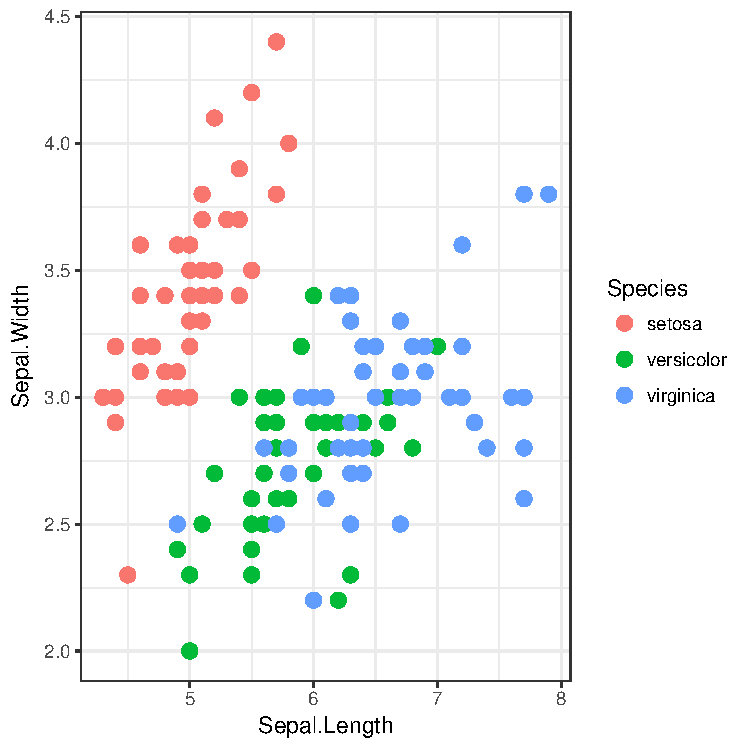
\includegraphics[width=6cm,height=6cm]{figure/iris_data-1} 
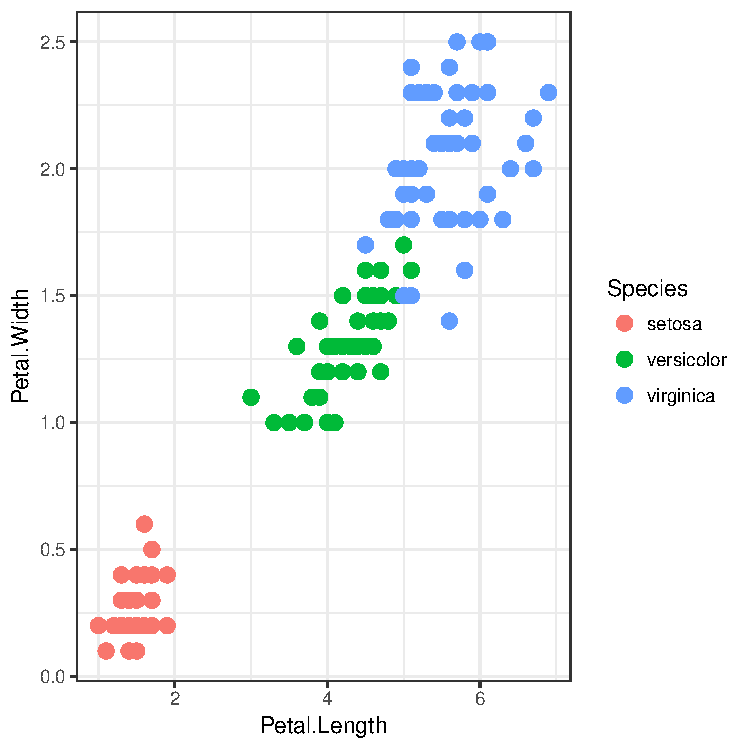
\includegraphics[width=6cm,height=6cm]{figure/iris_data-2} 
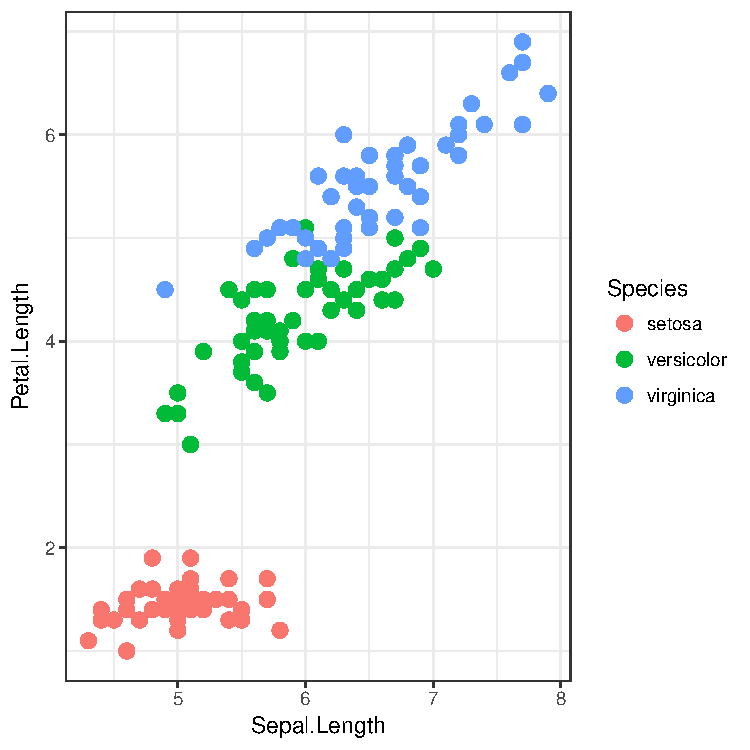
\includegraphics[width=6cm,height=6cm]{figure/iris_data-3} 
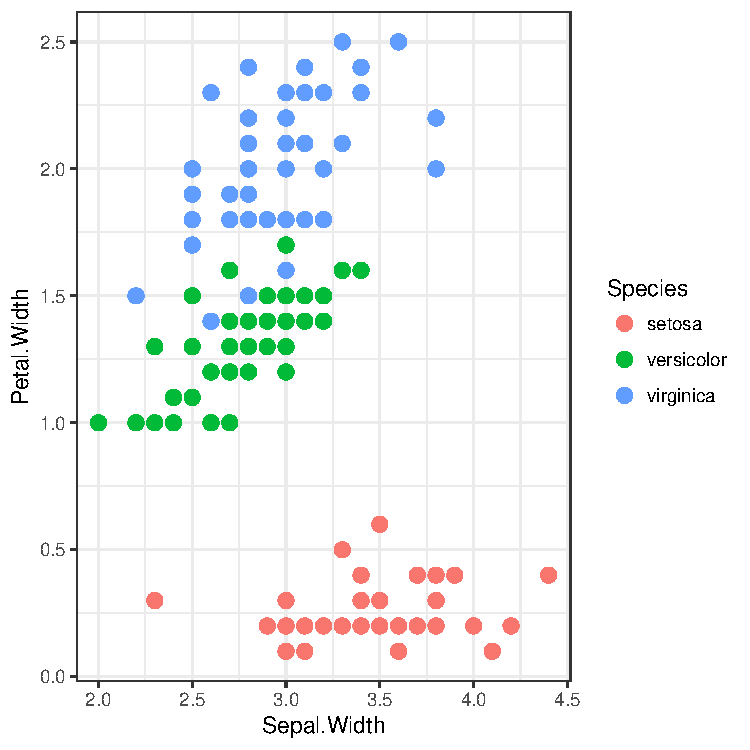
\includegraphics[width=6cm,height=6cm]{figure/iris_data-4} 
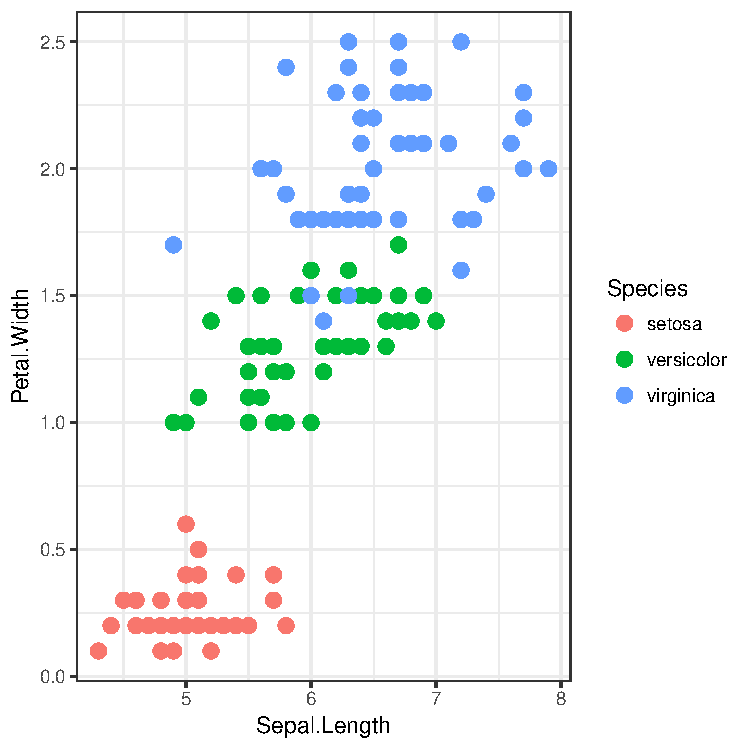
\includegraphics[width=6cm,height=6cm]{figure/iris_data-5} 
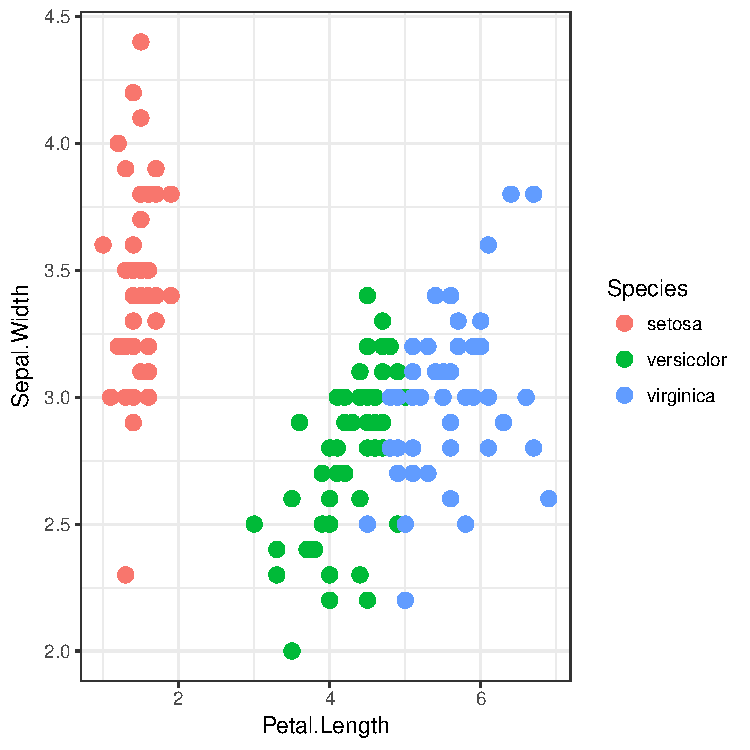
\includegraphics[width=6cm,height=6cm]{figure/iris_data-6} 

}



\end{knitrout}

\begin{knitrout}\small
\definecolor{shadecolor}{rgb}{0.969, 0.969, 0.969}\color{fgcolor}\begin{kframe}
\begin{alltt}
\hlstd{R> }\hlstd{(mod} \hlkwb{<-} \hlkwd{iprobit_mult}\hlstd{(y, X,} \hlkwc{silent} \hlstd{=} \hlnum{TRUE}\hlstd{))}
\end{alltt}
\begin{verbatim}
## Lower bound value =  -55.60715 
## Iterations =  100 
## 
##           Class = 1 Class = 2 Class = 3
## Intercept  -0.21708   1.20009  -1.13551
## lambda     -0.35226  -0.35226  -0.35226
\end{verbatim}
\begin{alltt}
\hlstd{R> }\hlkwd{plot}\hlstd{(mod)}
\end{alltt}
\end{kframe}

{\centering 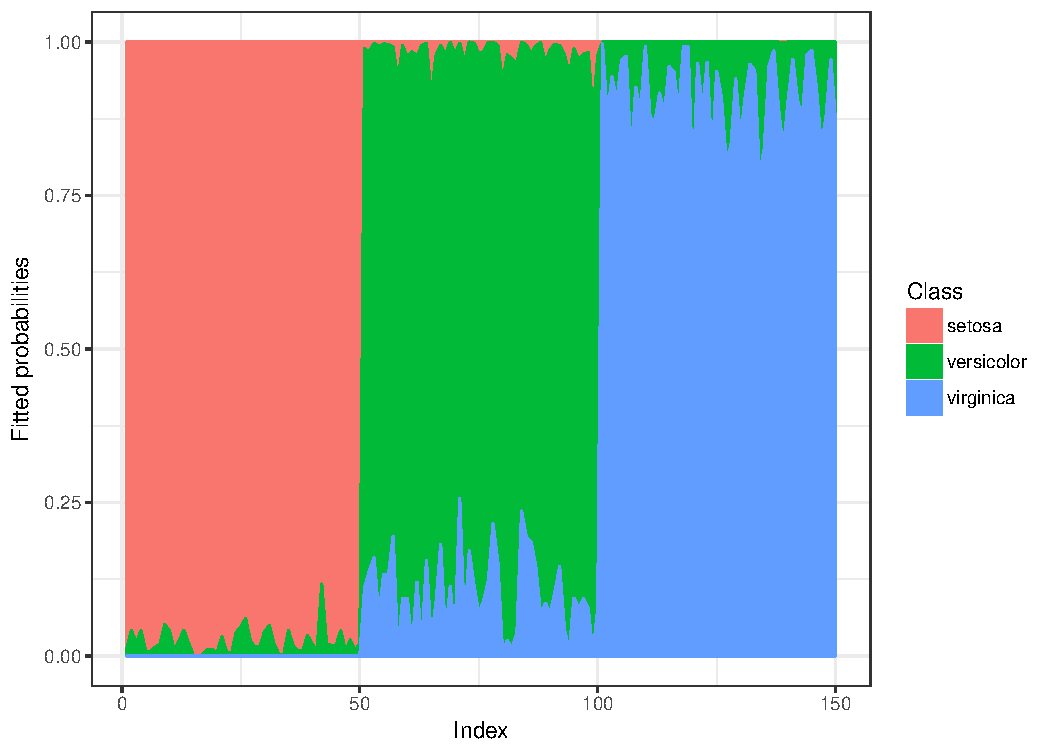
\includegraphics[width=\maxwidth]{figure/iris_mod-1} 

}


\begin{kframe}\begin{alltt}
\hlstd{R> }\hlkwd{iplot_lb}\hlstd{(mod)}
\end{alltt}
\end{kframe}

{\centering 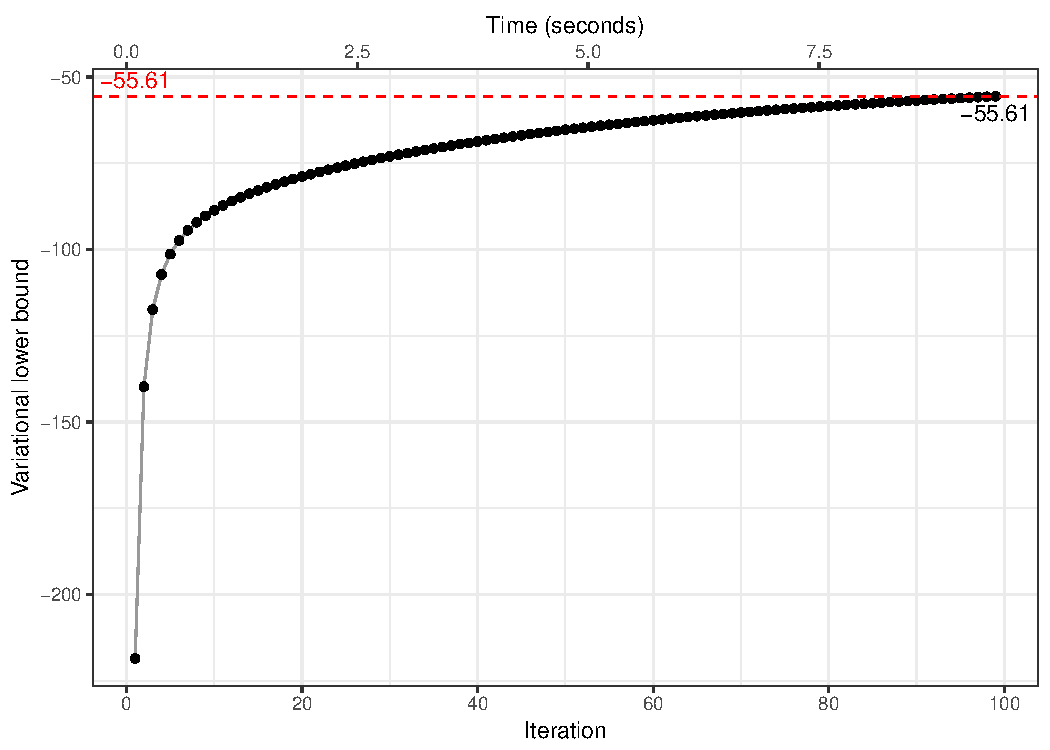
\includegraphics[width=\maxwidth]{figure/iris_mod-2} 

}



\end{knitrout}

\subsection{Vowel recognition data set}

\begin{knitrout}\small
\definecolor{shadecolor}{rgb}{0.969, 0.969, 0.969}\color{fgcolor}\begin{kframe}
\begin{verbatim}
##   class    x.1   x.2    x.3   x.4    x.5   x.6    x.7    x.8    x.9   x.10
## 1     1 -3.639 0.418 -0.670 1.779 -0.168 1.627 -0.388  0.529 -0.874 -0.814
## 2     2 -3.327 0.496 -0.694 1.365 -0.265 1.933 -0.363  0.510 -0.621 -0.488
## 3     3 -2.120 0.894 -1.576 0.147 -0.707 1.559 -0.579  0.676 -0.809 -0.049
## 4     4 -2.287 1.809 -1.498 1.012 -1.053 1.060 -0.567  0.235 -0.091 -0.795
## 5     5 -2.598 1.938 -0.846 1.062 -1.633 0.764  0.394 -0.150  0.277 -0.396
## 6     6 -2.852 1.914 -0.755 0.825 -1.588 0.855  0.217 -0.246  0.238 -0.365
\end{verbatim}
\end{kframe}
\end{knitrout}
\begin{knitrout}\small
\definecolor{shadecolor}{rgb}{0.969, 0.969, 0.969}\color{fgcolor}\begin{kframe}
\begin{alltt}
\hlstd{R> }\hlkwd{set.seed}\hlstd{(}\hlnum{123}\hlstd{)}
\hlstd{R> }\hlstd{(mod} \hlkwb{<-} \hlkwd{iprobit_mult}\hlstd{(vow.tr}\hlopt{$}\hlstd{class, vow.tr[,} \hlopt{-}\hlnum{1}\hlstd{],} \hlkwc{kernel} \hlstd{=} \hlstr{"FBM"}\hlstd{,} \hlkwc{silent} \hlstd{=} \hlnum{TRUE}\hlstd{))}
\end{alltt}
\begin{verbatim}
## Lower bound value =  -736.8918 
## Iterations =  100 
## 
##           Class = 1 Class = 2 Class = 3 Class = 4 Class = 5 Class = 6
## Intercept  -0.11514   0.13838   0.04304   0.07129   0.21767   0.46536
## lambda     -0.13430  -0.13430  -0.13430  -0.13430  -0.13430  -0.13430
##           Class = 7 Class = 8 Class = 9 Class = 10 Class = 11
## Intercept   0.40117   -0.3387   0.47458   -0.06605    0.67874
## lambda     -0.13430   -0.1343  -0.13430   -0.13430   -0.13430
\end{verbatim}
\begin{alltt}
\hlstd{R> }\hlkwd{plot}\hlstd{(mod)}
\end{alltt}
\end{kframe}

{\centering 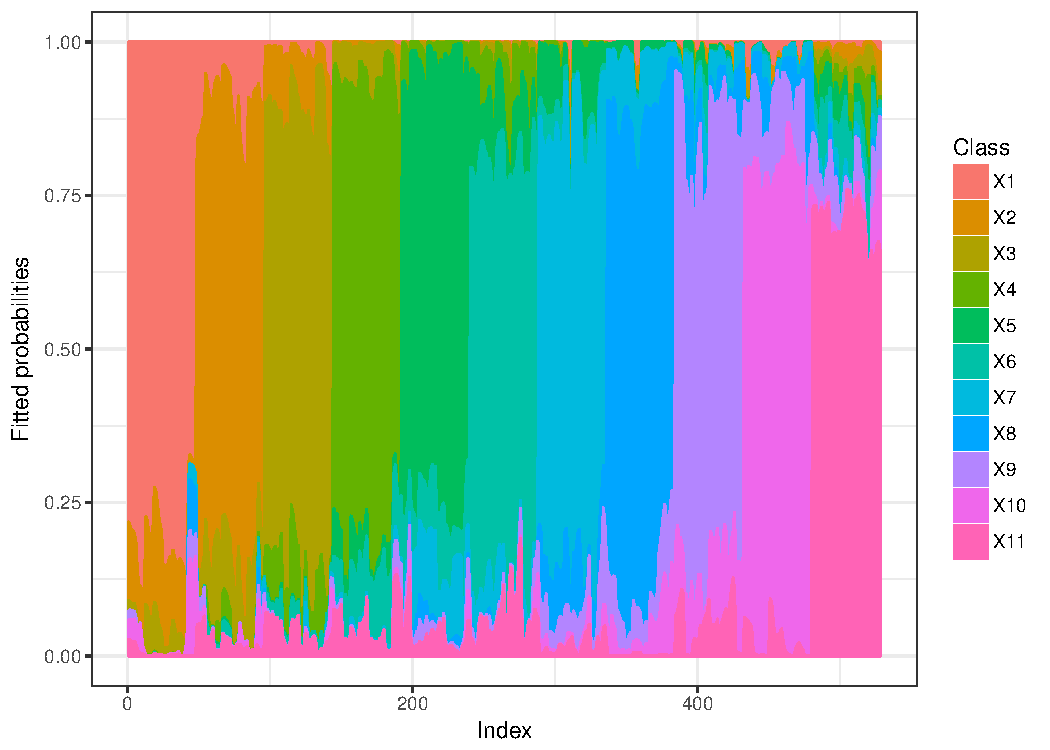
\includegraphics[width=\maxwidth]{figure/vowel_mod-1} 

}


\begin{kframe}\begin{alltt}
\hlstd{R> }\hlkwd{predict}\hlstd{(mod,} \hlkwc{X.test} \hlstd{= vow.ts[,} \hlopt{-}\hlnum{1}\hlstd{],} \hlkwc{y.test} \hlstd{= vow.ts[,} \hlnum{1}\hlstd{])}
\end{alltt}
\begin{verbatim}
## Test error rate: 41 %
\end{verbatim}
\end{kframe}
\end{knitrout}
\begin{table}[!h]
\centering
\begin{tabular}{lrr}
\toprule
\multicolumn{1}{c}{ } & \multicolumn{2}{c}{Error rates} \\ \cmidrule(l{2pt}r{2pt}){2-3}
  & Training & Test\\
\midrule
k-Nearest neighbours & NA & 44\\
Linear regression & 48 & 67\\
Linear discriminant analysis & 32 & 56\\
Neural network & NA & 45\\
FDA/BRUTO & 6 & 44\\
\addlinespace
FDA/MARS & 13 & 39\\
I-probit (FBM-0.5) & 0 & 41\\
\bottomrule
\end{tabular}
\end{table}



\end{document}




\section{Discussion}

\subsection{Estimating a scaled probit model}

\hltodo{For future work, can consider estimating the covariances/correlations across choices. More suitable for social science data.}

\subsection{Reduction to binary models}

\hltodo{Describe the model when there are only two alternatives.}

\subsection{Multiple scale parameters with multiple kernels}

\hltodo{It's definitely possible to extend to multiple scale parameters. It's just a matter of algebra.}

\subsection{Modelling ordinal data}

\hltodo{A different model using thresholds, but it might be possible to model these and estimate using variational inference.}

%%%%%%%%%%%%%%%%%%%%%%%%%%%%%%%%%%%%%%%%%%%%%%%%%%%%%%%%%%%%%%%%%%%%%%%%%%%%%%%%
%%% APPENDIX \%%%%%%%%%%%%%%%%%%%%%%%%%%%%%%%%%%%%%%%%%%%%%%%%%%%%%%%%%%%%%%%%%%
%%%%%%%%%%%%%%%%%%%%%%%%%%%%%%%%%%%%%%%%%%%%%%%%%%%%%%%%%%%%%%%%%%%%%%%%%%%%%%%%
\appendix

\section{Proofs}

\subsection{Proof of Lemma \ref{lem:expectation-entropy-truncated-mvn}}

\begin{proof}
\begin{enumerate}[label=(\roman*)]
  \item Due to the independence structure in the pdf of $\bX$, it is easy to consider the expectations of each of the components separately and marginalising out the rest of the components. For $i \neq j$, we have
  \begin{align*}
    \E[x_i] 
    &= C^{-1} \idotsint \ind[x_k < x_j, \forall k \neq j] \cdot x_i  \prod_{k=1}^d \frac{1}{\sigma_k}\phi \left( \frac{x_k - \mu_k}{\sigma_k} \right) \d x_1 \cdots \d x_d \\
    &= C^{-1} \iint \ind[x_i < x_j] \frac{x_i}{\sigma_i} \, \phi \left( \frac{x_i - \mu_i}{\sigma_i} \right)  \prod_{k \neq i,j} \Phi \left( \frac{x_j - \mu_k}{\sigma_k} \right) \frac{1}{\sigma_j}\phi \left( \frac{x_j - \mu_j}{\sigma_j} \right) \d x_i \d x_j \\
    &= C^{-1} \iint \ind[\sigma_i z_i + \mu_i < \sigma_j z_j + \mu_j] (\sigma_i z_i + \mu_i) \phi (z_i)  \prod_{k \neq i,j} \Phi \left( \frac{\sigma_j z_j + \mu_j - \mu_k}{\sigma_k} \right) \phi (z_j) \d z_i \d z_j \\
    &= \mu_i C^{-1} \iint \ind[ z_i < (\sigma_j z_j + \mu_j - \mu_i) / \sigma_i] \phi (z_i)  \prod_{k \neq i,j} \Phi \left( \frac{\sigma_j z_j + \mu_j - \mu_k}{\sigma_k} \right) \phi (z_j) \d z_i \d z_j \\*    
    &\phantom{==} + \sigma_i C^{-1} \iint \ind[z_i < (\sigma_j z_j + \mu_j - \mu_i) / \sigma_i] z_i \phi (z_i)  \prod_{k \neq i,j} \Phi \left( \frac{\sigma_j z_j + \mu_j - \mu_k}{\sigma_k} \right) \phi (z_j) \d z_i \d z_j \\
    &= \mu_i C^{-1} 
    \overbrace{
    \int  \prod_{k \neq j} \Phi \left( \frac{\sigma_j z_j + \mu_j - \mu_k}{\sigma_k} \right) \phi (z_j) \d z_j
    }^{C} \\  
    &\phantom{==} + \sigma_i C^{-1} \int \ind[ z_i < (\sigma_j z_j + \mu_j - \mu_i) / \sigma_i] z_i \phi (z_i) \prod_{k \neq i,j} \Phi \left( \frac{\sigma_j z_j + \mu_j - \mu_k}{\sigma_k} \right) \phi (z_j) \d z_i \d z_j \\
  \end{align*}
  The integral involving $z_i$ in the second part of the sum is recognised as the (unnormalised) expectation of the lower-tail of a univariate standard normal distribution truncated at $\tau_{ij} = (\sigma_j z_j + \mu_j - \mu_i) / \sigma_i$. That is,
  \[
    \E[Z_i | Z_i < \tau_{ij}] 
    = \big[\Phi(\tau_{ij})\big]^{-1} \int \ind [z_i < \tau_{ij}] z_i \phi(z_i) \d z_i 
    = - \frac{\phi(\tau_{ij})}{\Phi(\tau_{ij})}
  \] Plugging this expression back into the derivation of this expectation, we get
  \begin{align*}
  \E[X_i] 
  &= \mu_i -  \sigma_i C^{-1} \int 
  \phi \left( \frac{\sigma_j z_j + \mu_j - \mu_i}{\sigma_i} \right)
  \prod_{k \neq i,j} \Phi \left( \frac{\sigma_j z_j + \mu_j - \mu_k}{\sigma_k} \right) \phi (z_j) \d z_j \\
  &= \mu_i - \sigma_i C^{-1} \E \left[ \phi \left( \frac{\sigma_j Z_j + \mu_j - \mu_i}{\sigma_i} \right)
  \prod_{k \neq i,j} \Phi \left( \frac{\sigma_j Z_j + \mu_j - \mu_k}{\sigma_k} \right) \right].
  \end{align*}
  
  The expectation for the $j$th component is
  \begin{align*}
    \E[X_j] 
    &= C^{-1} \idotsint \ind[x_k < x_j, \forall k \neq j] \cdot x_j  \prod_{k=1}^d \frac{1}{\sigma_k}\phi \left( \frac{x_k - \mu_k}{\sigma_k} \right) \d x_1 \cdots \d x_d \\
    &= C^{-1} \int x_j  \prod_{k \neq j} \Phi \left( \frac{x_j - \mu_k}{\sigma_k} \right) 
    \cdot \frac{1}{\sigma_j} \phi \left( \frac{x_j - \mu_j}{\sigma_j} \right) \d x_j  \\    
    &= C^{-1} \int (\sigma_j z_j + \mu_j)  \prod_{k \neq j} \Phi \left( \frac{\sigma_j z_j + \mu_j - \mu_k}{\sigma_k} \right) \cdot \phi (z_j) \d z_j  \\   
    &= \mu_j C^{-1} 
    \overbrace{
    \int  \prod_{k \neq j} \Phi \left( \frac{\sigma_j z_j + \mu_j - \mu_k}{\sigma_k} \right) \cdot \phi (z_j) \d z_j
    }^{C}  \\   
    &\phantom{==} + \sigma_j C^{-1} \int  \prod_{k \neq j} \Phi \left( \frac{\sigma_j z_j + \mu_j - \mu_k}{\sigma_k} \right) \cdot z_j \phi (z_j) \d z_j \\
    &= \mu_j + \sigma_j C^{-1} \E \left[ Z_j \prod_{k \neq j} \Phi \left( \frac{\sigma_j Z_j + \mu_j - \mu_k}{\sigma_k} \right) \right] \\
    &= \mu_j + \sigma_j  \mathop{\sum_{i=1}^d}_{i \neq j} \sigma_i C^{-1} \E \Bigg[ \phi \left( \frac{\sigma_j Z_j + \mu_j - \mu_i}{\sigma_i} \right) \mathop{\prod_{k=1}^d}_{k \neq i,j} \Phi \left( \frac{\sigma_j Z_j + \mu_j - \mu_k}{\sigma_k} \right) \Bigg] \\
    &= \mu_j - \sigma_j \sum_{i \neq j} \big(\E[X_i] - \mu_i \big)
  \end{align*}
  where we have made use of Lemma \ref{lem:EZgZ} in the second last step of the above.

  \item The differential entropy is given by
  \begin{align*}
    \cH(p) &= -\int p(\bx) \log p(\bx) \d \bx = -\E \left[ \log p(\bx) \right] \\
    &= -\E \left[-\log C - \half[d] \log 2\pi - \half \sum_{i=1}^d \log \sigma_i^2 - \half \sum_{i=1}^d \left( \frac{x_i - \mu_i}{\sigma_i} \right)^2 \right] \\
    &= \log C + \half[d] \log 2\pi + \half \sum_{i=1}^d \log \sigma_i^2 + \half \sum_{i=1}^d \frac{1}{\sigma_i^2} \E [ x_i - \mu_i ]^2.
  \end{align*}
\end{enumerate}  
\end{proof}

\begin{lemma}\label{lem:EZgZ}
  Let $Z \sim \N(0,1)$. Then for all $m \in \{\bbN \, | \, m > 1\}$ and $(\mu, \sigma) \in \bbR \times \bbR^+$, 
  \[
    \E \Bigg[ Z \mathop{\prod_{k=1}^m}_{k \neq j} \Phi(\sigma_k Z + \mu_k) \Bigg]
    = \mathop{\sum_{i=1}^m}_{i \neq j} \E \Bigg[ \sigma_i \phi(\sigma_i Z + \mu_i) \mathop{\prod_{k=1}^m}_{k \neq i,j} \Phi (\sigma_k Z + \mu_k) \Bigg]
  \]
  for some $j \in \{1, \dots, m\}$.
\end{lemma}

\begin{proof}
  Use the fact that for any differentiable function $g$, $\E[Zg(Z)] = \E[g'(Z)]$, and apply the result with the function $g_m:z \mapsto \prod_{k \neq j} \Phi(\sigma_k z + \mu_k)$. All that is left is to derive the derivative of $g$, and we use an inductive proof to do this. 
  
  We adopt the following notation for convenience:
  \begin{align*}
    \phi_i = \phi(\sigma_i z + \mu_i) \\
    \Phi_i = \Phi(\sigma_i z + \mu_i) 
  \end{align*}
  
  The simplest case is when $m=2$, which can be trivially shown to be true. Without loss of generality, let $j=1$. Then
  \begin{align*}
    g_2(z) &= \Phi_2 \\
    \Rightarrow g_2'(z) &= \sigma_2 \phi_2 = \mathop{\sum_{i=1}^2}_{i \neq 1} \Bigg[ \sigma_i \phi_i \mathop{\sum_{k=1}^2}_{k \neq 1,2} \Phi_k \Bigg].
  \end{align*}
  
  Now assume that the inductive hypothesis holds for some $m \in \{\bbN \, | \, m > 1\}$. That is, the derivative of
  \[
    g_m(z) = \mathop{\prod_{k=1}^m}_{k \neq j} \Phi_k
  \]
  which is
  \[
    g_m'(z) = \mathop{\sum_{i=1}^m}_{i \neq j} \bigg[  \sigma_i \phi_i \mathop{\prod_{k=1}^m}_{k \neq i,j} \Phi_k \bigg],
  \]
  is assumed to be true. Assume that without loss of generality, $j \neq m+1$. Then the derivative of
  \[
    g_{m+1}(z) = \mathop{\prod_{k=1}^{m+1}}_{k \neq j} \Phi_k = g_m(z) \Phi_{m+1}
  \]
  is found to be
  \begin{align*}
    g_{m+1}'(z) &= \sigma_{m+1} \phi_{m+1} g_m(z) + g_m'(z) \Phi_{m+1} \\
    &= \sigma_{m+1} \phi_{m+1} \mathop{\prod_{k=1}^m}_{k \neq j} \Phi_k + \mathop{\sum_{i=1}^m}_{i \neq j} \bigg[  \sigma_i \phi_i \mathop{\prod_{k=1}^m}_{k \neq i,j} \Phi_k \bigg] \Phi_{m+1} \\
    &= \sigma_{m+1} \phi_{m+1} \mathop{\prod_{k=1}^{m+1}}_{k \neq j, m+1} \Phi_k + \mathop{\sum_{i=1}^m}_{i \neq j} \bigg[  \sigma_i \phi_i \mathop{\prod_{k=1}^{m+1}}_{k \neq i,j} \Phi_k \bigg] \\
    &= \mathop{\sum_{i=1}^{m+1}}_{i \neq j} \bigg[  \sigma_i \phi_i \mathop{\prod_{k=1}^{m+1}}_{k \neq i,j} \Phi_k \bigg] \\
    &= g_{m+1}'(z).
  \end{align*}
  Thus, by induction and linearity of expectations, the proof is complete.
\end{proof}

%\begin{lemma}
%  Let $Z \sim \N(0,1)$. Then
%  \[
%    \E[Z\Phi(\mu + \sigma Z)] = \E[\sigma \phi(\mu + \sigma z)].
%  \]
%\end{lemma}
%
%\begin{proof}
%  Use the fact that for any differentiable function $g$, $\E[Zg(Z)] = \E[g'(Z)]$, and apply the function $g:z \mapsto \Phi(\mu + \sigma z)$ with derivative $g'(z) = \sigma \phi(\mu + \sigma z)$.
%\end{proof}

%%%%%%%%%%%%%%%%%%%%%%%%%%%%%%%%%%%%%%%%%%%%%%%%%%%%%%%%%%%%%%%%%%%%%%%%
%%% REFERENCES %%%%%%%%%%%%%%%%%%%%%%%%%%%%%%%%%%%%%%%%%%%%%%%%%%%%%%%%%
%%%%%%%%%%%%%%%%%%%%%%%%%%%%%%%%%%%%%%%%%%%%%%%%%%%%%%%%%%%%%%%%%%%%%%%%
\ifstandalone
  {
  \nocite{Albert1993, Dow2004, Sheffi1982, Natarajan1995, Bolduc1999, Rogers2007, Girolami2006}
  \printbibliography
  }
\fi
\end{document}















